\documentclass[a4paper,12pt]{report}

\usepackage[T1]{fontenc}
\usepackage[utf8]{inputenc}
\usepackage[english]{babel}

\usepackage[hidelinks]{hyperref}
\usepackage{graphicx}
\usepackage{caption}
\usepackage{subcaption}

\title{Connector - Reference manual }
\author{Gianluigi Forte}

\usepackage{listings}
\usepackage{color}

\lstdefinelanguage{asymptote}{%
keywords=[1]{import, unitsize, add, shift,
 show, arc, include}, %pour asymptote + geometry
keywords=[2]{label, draw, dot, geometry, grid, triangleabc, perpendicularmark},% pour les autres extensions
keywords=[3]{pair, triangle, path}, % pour les classes
keywords=[4]{lightgray, black, gray, red}, %pour les couleurs
keywords=[5]{bp, pt, cm,  % unités
 N, E, S, W, NE, SE, SW, NW,
 NNE, ENE, ESE, SSE, SSW, WSW, WNW, NNW},% points cardinaux
comment=[l]{//},
otherkeywords={ -- , .. , :: , \^\^},
sensitive=true,
%morecomment=[s]{/*}{*/},
%string=[d]",
moredelim=*[s][\color{black}]{"}{"},
moredelim=**[s][\color{black}]{{$}{$}}
}


\lstset{%
language=asymptote,
keywordstyle=[1]\ttfamily\bfseries\color{black},
keywordstyle=[2]\ttfamily\color{black},
keywordstyle=[3]\ttfamily\bfseries,
keywordstyle=[4]\ttfamily\color{black},
keywordstyle=[5]\ttfamily\bfseries\color{black},
identifierstyle=\ttfamily\color{black},
firstnumber=5
}% à compléter au besoin
%
%

\begin{document}
\maketitle

\section*{Introduction}

Connector is a library written in \emph{Asymptote} language to generate figures of electronic schematics. \LaTeX and \emph{Asymptote}, differently from other programs like Word or Write, are languages designed to produce documents with the best quality outputs for prints or presentations starting from a description, of the content to be produced, expressed programmatically in a source code text file and then produced in output after the compilation process. The idea behind the \emph{connector} library is to provide a ready to use set of functions written in Asymptote language to draw electrical components, link them with connection (wires), decorate with labels and produce the output figure as pdf or png files to be embedded in a larger Latex document or any kind of other usage like websites, videos, presentations and so on. An example of the image generated with \emph{connector} is shown in figure \ref{threePhaseInverterExample}. The source code \texttt{ThreePhaseInverter.asy} to produce the figure is included in the library.

\begin{figure}[ht]
  \centering
  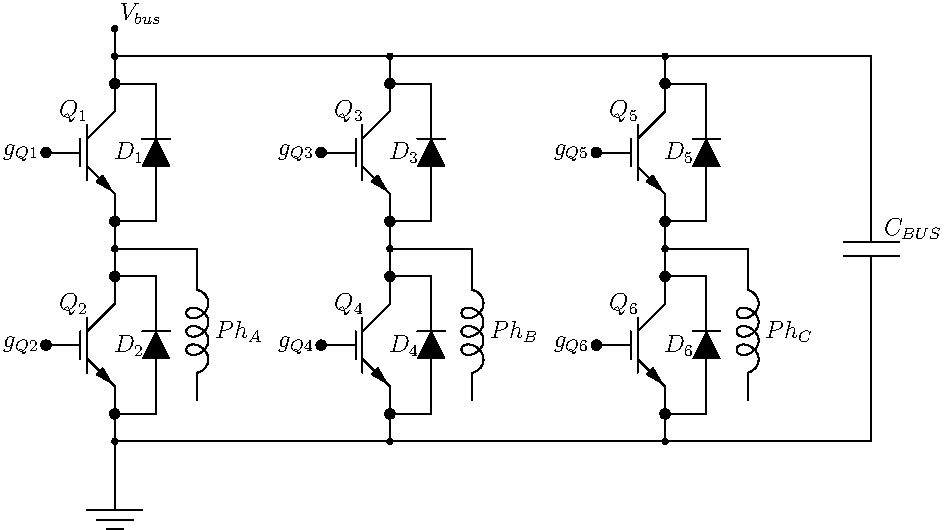
\includegraphics[width=1.0\textwidth]{ThreePhaseInverter.pdf}
  \caption{Example of schematics generated with \emph{connector}}
  \label{threePhaseInverterExample}
\end{figure}

\section*{Getting started}

Before to use the \emph{Connector} library is necessary to install the \emph{Asymptote } compiler. Follow the instruction described in the \emph{Asymptote} website at this \href{https://asymptote.sourceforge.io}{link}. It is required to install the \LaTeX environment as mentioned in the \emph{Asymptote} installation documentation. It is also suggested to install \emph{Node.JS} (\href{https://nodejs.org}{link}) to execute the script \texttt{watch.js} that is able to generate automatically the output of the \emph{.asy} file you are working every time you modify it. Finally, it is also kindly suggested to install \emph{Visual Studio Code} (\href{https://code.visualstudio.com}{link}) and some of its fantastic extensions to support \emph{Asymptote} and \LaTeX languages.

Download and unpack the \emph{Connector} library in a working folder of your file system, take a look at the examples \texttt{.asy} file that are provided to take inspiration. Create a \texttt{newFile.asy} with your code and compile it with the command line \texttt{asy newFile.asy}. The compiled \texttt{.pdf} file will be created in the current folder. Or use \texttt{node watch.js newFile.asy} for the automatic generation after each file modification. The compiled \texttt{.pdf} file will be created in the \texttt{generated} folder in this case. It is possible to produce a \texttt{.png} file adding the line \texttt{settings.outformat="png";} to your code or replacing the line \texttt{settings.outformat="pdf"} with \texttt{"png"} if it is already present.

It is also kindly suggested to learn the \emph{Asymptote} language to be familiar with the \emph{Connector} library and to use it at the best.

If you want to collaborate with the \emph{Connector} project to add other symbols, for the internationalization of the documentation, to fix or report some bugs, to request other features, or for any other kind of collaborations, please let me know at \emph{\href{mailto:koalakoker@gmail.com}{koalakoker@gmail.com}}.

\section*{Electronic Symbols}

The following list of components have been included in the library and can be used out-of-the-box: node, resistor, capacitor, inductor, fuse, diode, relay, relay SPDT, IGBT, MOS, power ground, signal ground. Maybe other will be added in the future.

In the figures from \ref{fig:nodeInfo} to \ref{fig:gndSignalInfo} are shown the components, the anchor points as a black dot. The anchor point direction is indicated with a green line starting from the dot and going outward, the anchor point index number is indicated near the end of the green line. It is also indicated the position of the pivot point $(0,0)$ and also the position of the $(1,0)$ point for a spatial reference; both are indicated with a red cross.

In figure \ref{fig:nodeInfo} is shown a generic node symbol. See \texttt{nodeInfo.asy} code to reproduce the figure. Note that this symbol has four anchor points going in four different directions. It can be very useful to connect different part of the schematics with a connector line.

To draw any symbol without the indication of the anchor points, pivot point and all other info simply call the \texttt{draw} method without the \texttt{drawOpt} parameter or setting it to \texttt{null}.   

\begin{figure}[ht]
\centering
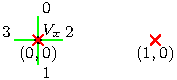
\includegraphics[width=0.4\textwidth]{nodeInfo}
\caption{Generic node symbol}
\label{fig:nodeInfo}
\end{figure}

In figure \ref{fig:resistorInfo} is shown the resistor symbol. See \texttt{resistorInfo.asy} code to reproduce the figure.

\begin{figure}[ht]
\centering
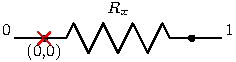
\includegraphics[width=0.4\textwidth]{resistorInfo}
\caption{Resistor symbol}
\label{fig:resistorInfo}
\end{figure}

In figure \ref{fig:capaciorInfo} is shown the capacitor symbol. See \texttt{capaciorInfo.asy} code to reproduce the figure.

\begin{figure}[ht]
\centering
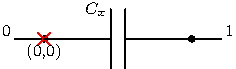
\includegraphics[width=0.4\textwidth]{capacitorInfo}
\caption{Capacitor symbol}
\label{fig:capaciorInfo}
\end{figure}

In figure \ref{fig:inductorInfo} is shown an inductor symbol. See \texttt{inductorInfo.asy} code to reproduce the figure.

\begin{figure}[ht]
\centering
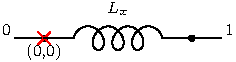
\includegraphics[width=0.4\textwidth]{inductorInfo}
\caption{Inductor symbol}
\label{fig:inductorInfo}
\end{figure}

In figure \ref{fig:fuseInfo} is shown the fuse symbol. See \texttt{fuseInfo.asy} code to reproduce the figure.

\begin{figure}[ht]
\centering
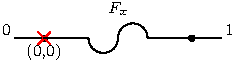
\includegraphics[width=0.4\textwidth]{fuseInfo}
\caption{Fuse symbol}
\label{fig:fuseInfo}
\end{figure}

In figure \ref{fig:diodeInfo} is shown the diode symbol. See \texttt{diodeInfo.asy} code to reproduce the figure.

\begin{figure}[ht]
\centering
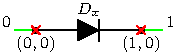
\includegraphics[width=0.4\textwidth]{diodeInfo}
\caption{Diode symbol}
\label{fig:diodeInfo}
\end{figure}

In figure \ref{fig:relayInfo} is shown the relay symbol. See \texttt{relayInfo.asy} code to reproduce the figure.

\begin{figure}[ht]
\centering
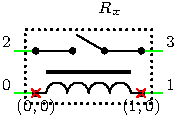
\includegraphics[width=0.35\textwidth]{relayInfo}
\caption{Relay symbol}
\label{fig:relayInfo}
\end{figure}

In figure \ref{fig:relaySPDTInfo} is shown the relay SPDT symbol. See \texttt{relaySPDTInfo.asy} code to reproduce the figure.

\begin{figure}[ht]
\centering
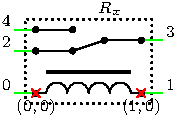
\includegraphics[width=0.35\textwidth]{relaySPDTInfo}
\caption{Relay SPDT symbol}
\label{fig:relaySPDTInfo}
\end{figure}

In figure \ref{fig:igbtInfo} is shown the IGBT symbol. See \texttt{igbtInfo.asy} code to reproduce the figure.

\begin{figure}[ht]
\centering
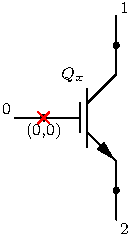
\includegraphics[width=0.3\textwidth]{igbtInfo}
\caption{Igbt symbol}
\label{fig:igbtInfo}
\end{figure}

In figure \ref{fig:mosInfo} is shown the MOSFET transistor symbol. See \texttt{mosInfo.asy} code to reproduce the figure.

\begin{figure}[ht]
\centering
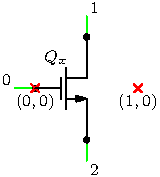
\includegraphics[width=0.3\textwidth]{mosInfo}
\caption{MOSFET transistor symbol}
\label{fig:mosInfo}
\end{figure}

In figure \ref{fig:gndPowerInfo} is shown the power ground symbol. See \texttt{gndPowerInfo.asy} code to reproduce the figure.

\begin{figure}[ht]
\centering
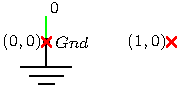
\includegraphics[width=0.3\textwidth]{gndPowerInfo}
\caption{Power ground symbol}
\label{fig:gndPowerInfo}
\end{figure}

In figure \ref{fig:gndSignalInfo} is shown the signal ground symbol. See \texttt{gndSignalInfo.asy} code to reproduce the figure.

\begin{figure}[ht]
\centering
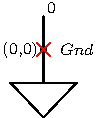
\includegraphics[width=0.3\textwidth]{gndSignalInfo}
\caption{Signal ground symbol}
\label{fig:gndSignalInfo}
\end{figure}

\clearpage
\section*{Symbol positioning and orientation}
For each symbol instantiated it is possible to define its placement in the drawing calling the methods \texttt{setPos} and passing the position of the pivot point as parameter before calling the \texttt{draw} method. For example, the code:
\begin{lstlisting}
  size(4cm);
  defaultpen(fontsize(8pt));
  import resistor;
  import drawOptions;
  Resistor r = Resistor();
  r.setPos((1,0));
  r.draw(DrawOption(showOrigin = true));
\end{lstlisting}
will draw the image shown in figure \ref{fig:placingExample1}. The same effect can be done passing the position of the pivot point as parameter in the constructor function \texttt{Resistor r = Resistor((1,0))}.
\begin{figure}[ht]
  \centering
  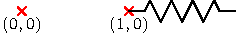
\includegraphics[width=0.5\textwidth]{placingExample1.pdf}
  \caption{Placing the pivot point of the symbol in $(1,0)$}
  \label{fig:placingExample1}
\end{figure}

In a similar way is possible to define the orientation of the symbol calling the methods \texttt{setOrient} and passing the orientation of the symbol around the pivot point as parameter before calling the \texttt{draw} method. For example, the code:
\begin{lstlisting}
  size(4cm);
  defaultpen(fontsize(8pt));
  import resistor;
  import drawOptions;
  Resistor r = Resistor();
  r.setOrient(90);
  r.draw(DrawOption(showOrigin = true));
\end{lstlisting}
will draw the image shown in figure \ref{fig:placingExample2}. The same effect can be done passing the orientation of the symbol around the pivot point as parameter in the constructor function \texttt{Resistor r = Resistor(orient = 90)}. The only valid options for the orient parameter are 0, 90, -90  and 180. The anchor points of the symbol will be re-oriented according to the orientation of the symbol.
\begin{figure}[ht]
  \centering
  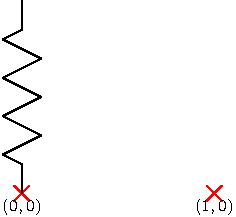
\includegraphics[width=0.35\textwidth]{placingExample2.pdf}
  \caption{Set the orientation of the symbol around the pivot point as 90}
  \label{fig:placingExample2}
\end{figure}

It is possible to use the same instance of the symbol to print it several times in different positions and/or different orientations. In this case can be useful to change the label of the printed instance using the method \texttt{setLabel} and passing the new label as parameter before calling the \texttt{draw} method. For example, the code:
\begin{lstlisting}
  size(4cm);
  defaultpen(fontsize(8pt));
  import components;
  import drawOptions;
  import connector;
  Resistor r = Resistor("$R_1$");
  Capacitor c = Capacitor((1,0), -90,"$C_1$");
  Node n = Node((0,-1.1));
  n.draw();
  r.draw(DrawOption(showOrigin = true));
  drawAnchorConnector(n, 2, c, 1);
  c.draw();
  r.setPos((1,0));
  r.setLabel("$R_2$");
  r.draw();
  c.setPos((2,0));
  c.setLabel("$C_2$");
  c.draw();
  drawAnchorConnector(n, 2, c, 1);
\end{lstlisting}
will draw the image shown in figure \ref{fig:placingExample3}.
\begin{figure}[ht]
  \centering
  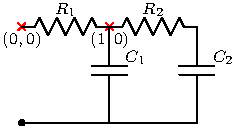
\includegraphics[width=0.5\textwidth]{placingExample3.pdf}
  \caption{Example of multiple symbol placement with the same instance}
  \label{fig:placingExample3}
\end{figure}

In figure \ref{fig:placingExample3} the $R_1$ and $R_2$ are drown using the same \emph{Resistor} instance $r$. In the same way $C_1$ and $C_2$ are drown using the same \emph{Capacitor} instance c. The \emph{Node} n is used to draw the connectors of the bottom of the figure. If the positioning of the symbol label is not perfect, it is possible to send a \emph{pair} as second parameter of the method \texttt{setLabel} to set a displacement position only for the label. 

\section*{Anchor points}
\label{sct:anchorPoints}

The anchor points are used to connect the symbol using \emph{Connectors} as described in section \nameref{sct:connector}. Each symbol has a set of anchor points already defined. Use figures from \ref{fig:nodeInfo} to \ref{fig:gndSignalInfo} as reference to know which anchor points are defined in the symbol.

An anchor point has a position indicated with a dot in the symbol figures, this will be the starting or ending point of the connectors. The anchor point has an index, indicated with a number in the symbol figures. This index will be used to identify the anchor point among the various present in the symbol. The anchor point has a direction indicated with the green line in the symbol figures, that start from the dot and go outward. This will be the direction of the connector that starts o ends in this specific anchor point.

It is possible to get the position of an anchor point of an instance of a symbol with the function \texttt{GetAnchorPos(obj, index)}. Each symbol is a derived class from a generic object. The function returns a \emph{pair} that indicate the coordinate of the anchor position; this can be used to place other symbols aligned with that position. Many examples provided with the library make use of this strategy to align the symbols. E.g., \texttt{ThreePhaseInverter.asy}.

It is possible to change the orientation of an anchor point with the function \texttt{setAnchorDirection(object, index, direction)}. Where \texttt{object} is the instance of the symbol on which operate, \texttt{index} is the index of the anchor point to be modified and \texttt{direction} is the new direction. The available directions are: \emph{DN} (equal to north or up), \emph{DS} (equal to south or down), \emph{DE} (equal to east or right) or \emph{DW} (equal to west or left). In figure \ref{fig:anchorPointExample} are shown respectively the outputs of the examples \texttt{anchorExample1.asy} \ref{subFig:anchorExampleDefault} and \texttt{anchorExample1.asy} \ref{subFig:anchorExampleCustom}. It is an example on how to customize the direction of the default anchor points. 

\begin{figure}
  \centering
  \begin{subfigure}{.4\textwidth}
    \centering
    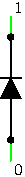
\includegraphics[width=0.1\linewidth]{anchorExample1.pdf}
    \caption{Default directions}
    \label{subFig:anchorExampleDefault}
  \end{subfigure}\hfill
  \begin{subfigure}{.4\textwidth}
    \centering
    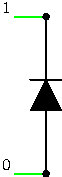
\includegraphics[width=0.2\linewidth]{anchorExample2.pdf}
    \caption{Custom directions}
    \label{subFig:anchorExampleCustom}
  \end{subfigure}\hfill
  \caption{Changing the anchor points default directions}
  \label{fig:anchorPointExample}
\end{figure}

It is also possible to add other anchor points to a symbol using the function \texttt{AddAnchorPoint(object, position, direction)}. Where \texttt{object} is the instance of the symbol on which operate, \texttt{position} is a \emph{pair} that defines the position of the new anchor point; note that this \texttt{position} is the absolute position of the anchor point in the drawing, while the relative position respects the parent symbol is computed by the function. And \texttt{direction} is the direction of the new anchor point. The available directions are, with the same meaning mentioned before: \emph{DN}, \emph{DS}, \emph{DE}, \emph{DW}. In figure \ref{fig:anchorExample3} is shown the output of the \texttt{anchorExample3.asy} code that shows how to add other anchor points to a symbol; this can be very useful to put different symbols in parallel.

\begin{figure}[ht]
  \centering
  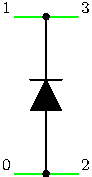
\includegraphics[width=0.14\textwidth]{anchorExample3.pdf}
  \caption{Adding new anchor points to a symbol}
  \label{fig:anchorExample3}
\end{figure}

\clearpage
\section*{Connectors}
\label{sct:connector}

It is possible to draw connectors (wires) between symbols with the function \texttt{drawAnchorConnector}. In particular the connection is done starting from one anchor point to another anchor point that are defined in the symbol. See from figure \ref{fig:nodeInfo} to figure \ref{fig:gndSignalInfo} to check the default anchor points defined in each symbol. See section \nameref{sct:anchorPoints} for details about anchor points. The path of the connector is automatically computed by the library in the best way and is drown according to the direction of the anchor point. The figure \ref{fig:connectorExample} show an example of connections between generic objects.

\begin{figure}[ht]
  \centering
  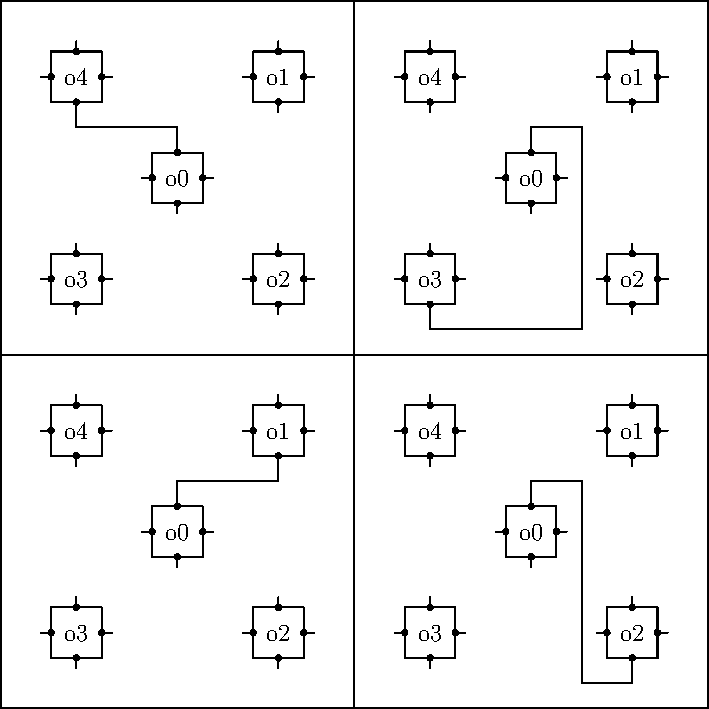
\includegraphics[width=1.0\textwidth]{N-S}
  \caption{Example of use of connectors between objects}
  \label{fig:connectorExample}
\end{figure}

The \texttt{drawAnchorConnector} function takes as parameters respectively: the first object to be connected, the anchor point index of the first object, the second object to be connected and the index of the anchor point of the second object.

\texttt{drawAnchorConnector(obj1, Anchor1, obj2, Anchor2)}

There are also other three optional parameters that can be used to set the aspect of the connection ($r_1,r_2,r_3$). As shown in figure \ref{fig:r1_connectorExample}, the $r_1$ parameter can be used to define the distance of the two corners of the connector line (and so the distance of the vertical line in figure \ref{fig:r1_connectorExample}). The parameter $r_1$ defines the distance of the first corner of the connector line from the first object expressed in percentage of the distance of the two objects.

\begin{figure}
  \centering
  \begin{subfigure}{.33\textwidth}
    \centering
    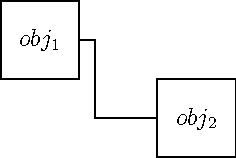
\includegraphics[width=0.9\linewidth]{connectorExample_r1_0_2.pdf}
    \caption{$r_1=0.2$}
  \end{subfigure}\hfill
  \begin{subfigure}{.33\textwidth}
    \centering
    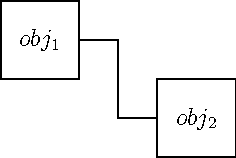
\includegraphics[width=0.9\linewidth]{connectorExample_r1_0_5.pdf}
    \caption{$r_1=0.5$}
  \end{subfigure}\hfill
  \begin{subfigure}{.33\textwidth}
    \centering
    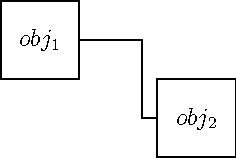
\includegraphics[width=0.9\linewidth]{connectorExample_r1_0_8.pdf}
    \caption{$r_1=0.8$}
  \end{subfigure}

  \caption{Effect of $r_1$ parameter value on connector}
  \label{fig:r1_connectorExample}
\end{figure}

The figure \ref{fig:r2_connectorExample} shows the $r_2$ parameters. It affects the distance between the second object and the first corner of the connector line.

\begin{figure}
  \centering
  \begin{subfigure}{.33\textwidth}
    \centering
    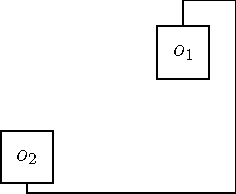
\includegraphics[width=0.9\linewidth]{connectorExample_r2_0_2.pdf}
    \caption{$r_2=0.2$}
  \end{subfigure}\hfill
  \begin{subfigure}{.33\textwidth}
    \centering
    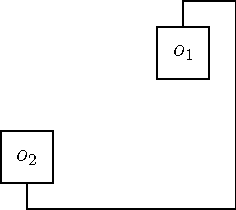
\includegraphics[width=0.9\linewidth]{connectorExample_r2_0_5.pdf}
    \caption{$r_2=0.5$}
  \end{subfigure}\hfill
  \begin{subfigure}{.33\textwidth}
    \centering
    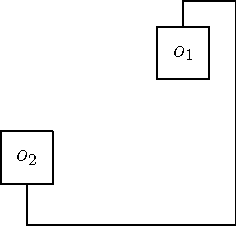
\includegraphics[width=0.9\linewidth]{connectorExample_r2_0_8.pdf}
    \caption{$r_2=0.8$}
  \end{subfigure}

  \caption{Effect of $r_2$ parameter value on connector}
  \label{fig:r2_connectorExample}
\end{figure}

The figure \ref{fig:r3_connectorExample} shows the $r_3$ parameters. It affects the distance between the first corner and the second corner (or equivalently the distance of the vertical bar) of the connector line.

\begin{figure}
  \centering
  \begin{subfigure}{.33\textwidth}
    \centering
    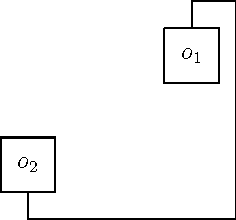
\includegraphics[width=0.9\linewidth]{connectorExample_r3_0_8.pdf}
    \caption{$r_3=0.8$}
  \end{subfigure}\hfill
  \begin{subfigure}{.33\textwidth}
    \centering
    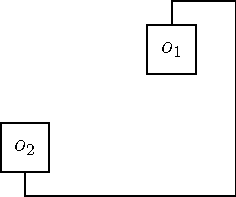
\includegraphics[width=0.9\linewidth]{connectorExample_r3_1_3.pdf}
    \caption{$r_3=1.3$}
  \end{subfigure}\hfill
  \begin{subfigure}{.33\textwidth}
    \centering
    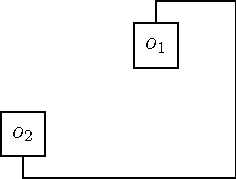
\includegraphics[width=0.9\linewidth]{connectorExample_r3_1_8.pdf}
    \caption{$r_3=1.8$}
  \end{subfigure}

  \caption{Effect of $r_2$ parameter value on connector}
  \label{fig:r3_connectorExample}
\end{figure}

\end{document}